We selected Play Framework for numerous reasons one of the main reason is that because this framework is proven in production. LinkedIn web application for example has been developed using play! framework. The overview of overview of Play! framework components is shown in figure\ref{play}.\\

\begin{figure}[h]
\centering
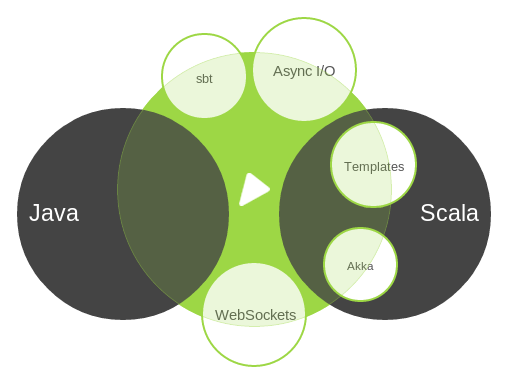
\includegraphics[scale=0.5]{./img/play.png}
\caption{\small{model,view and controller that are interconnected by directed edges}}
\label{play}
	
\end{figure}
 
Here We are going to mention some of our favorite features extracted from Play! documentation \cite{playDoc} that can help us to achieve our desired technical objectives. It is an open source application that has an amazing error handling because everything is compiled and built. This make it easy for developers to detect bugs and can dramatically improve developer's productivity to make a change. If you hit reload button on browser you can immediately see changes on the browser and is great feature for fast prototyping for our project. Moreover Play! has a great documentation and it supports Scala and Java language. It comes with a handy Scala template to write dynamic codes on HTML body. It also comes with pre-configured testing support, this is important because we then no need to worry about adding dependencies to the build file.\\
It also comes with the EBean server interface that makes in easy for fetching and saving beans to a particular DataSource. pLAY FRAMEWORK can make reactive application program more simple Because play is built on Netty, that means it supports non-blocking I/O. This will enable our web application to make remote calls inexpensively which is important for high performance web applications.






